\section{\label{sec:aufbau}Aufbau und Durchführung}
\subsection{\label{subsec:vers1}Röntgenstrahlabsorption}
Im ersten Teil des Versuchs charakterisieren wir das Material einer absorbierenden Metallfolie anhand 
der Absorptionskanten, die wir im Röntgenspektrum messen. Der Versuchsaufbau ist in Abb.~\ref{fig:vers1}
dargestellt.
\begin{figure}[h!]
    \centering
    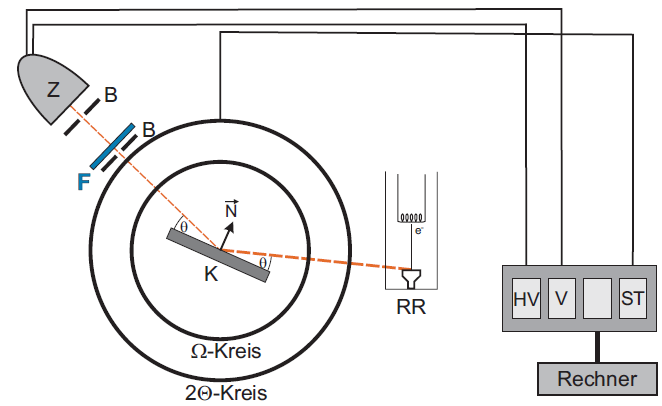
\includegraphics[width=0.73\textwidth]{Aufbau1.png}
    \caption{Skizze des Versuchsaufbaus zur Röntgenstrahlabsorption. Die Hauptbestandteile und deren 
    Funktionsweise sind im Haupttext beschrieben. Die Grafik wurde der Versuchsanleitung entnommen \cite{Anleitung}.}
    \label{fig:vers1}
\end{figure}\FloatBarrier
Die Röntgenstrahlung wird mithilfe einer Wolfram-Anode erzeugt, deren Funktionsweise 
sowie das entstehende weiße Spektrum in der vorbereitenden 
Frage \ref{subsec:FZV1} diskutiert wird. Über die Spannung $U$ zwischen Anode und 
Kathode, sowie den Strom $I$ in der Kathode kann die Energie und die Anzahl der 
Röntgenphotonen eingestellt werden. \\
Die Röntgenstrahlung fällt auf einen Einkristall (K), dessen Orientierung 
durch den Winkel $\Omega$ eingestellt werden kann. Auf einer davon unabhängigen 
Schiene befindet ein Proportionalzählrohr, das als Detektor der eintreffenden 
Röntgenphotonen dient. Die Position lässt sich über den $2\Theta$-Kreis einstellen. 
Vor dem Detektor befinden sich Blenden, die störende Untergrundsignale 
verringern. \\
Verwendet wird ein kubisch-flächenzentrierter $CaF_{2}$-Kristall mit 
einem Gitterparameter von $a= 5,463\pm 0,001\,\si{\angstrom}$, wobei 
der Strahl an der (220)-Netzebene gebeugt wird. \\
Nach richtiger Justage wir die Intensität (Anzahl der gebeugten Photonen) in 
Abhängigkeit des Einfallwinkels $\Theta$ aufgenommen. Hierzu wird der 
Einkristall und der Detektor schrittweise gedreht, wobei die Winkelschrittweite 
des Zählrohrs verdoppelt wird. Ein am Kristall gebeugtes Signal kann nur 
gemessen werden, wenn Einfalls- und Ausfallswinkel übereinstimmen, da 
sonst aufgrund unterschiedlicher Phasendifferenzen keine Interferenz beobachtbar
ist. \\ \\
Vor der eigentlichen Messung wird die Kristall- und Zählerposition justiert. 
Hierzu wird zunächst der Winkel $\Omega$ gesucht, für den der Strahl parallel
wird, was zu einem Intensitätsmaximum führt. Für erhöhte Genauigkeit wird
zunächst das Intensitätsmaximum gesucht und hiernach die Winkel, an denen die halbe 
Maximalintensität erreicht wird. Um den Detektor vor Übersättigung zu schützen, 
wird ein Metallstück in den Strahlengang eingebaut. Nachdem die optimale Stellung 
des Kristalls erreicht ist, wird mit gleichem Verfahren das Zählrohr verfahren, 
damit der Strahl mittig in den Detektorspalt fällt. Die ermittelten Winkel werden
im Steuerprogramm am Rechner eingepflegt. \\ \\
Für die Messungen stellen wir an der Röntgenröhre $I = 40\,\si{mA}$ und 
$U = 50\,\si{kV}$ ein. Zunächst wird im vorderen Winkelbereich 
$\Theta\,\in\,[5,0^{\circ},\,29,0^{\circ}]$ mit einer Schrittweite von 
$\Delta{\Theta} = 0,020^{\circ}$ gemessen, wobei die gezählten Signale 
über eine Integrationszeit von $t=1,5\,\si{s}$ aufsummiert werden. 
Im hinteren Winkelbereich $\Theta\,\in\,[22,5^{\circ},\,51,0^{\circ}]$
wird die Integrationszeit auf $t=5\,\si{s}$ erhöht. 
Diese Messung wird jeweils mit und ohne Absorberfolie (Nummer 6) durchgeführt, 
womit der erste Teil der Versuchs abgeschlossen ist. \\

\subsection{\label{subsec:vers2}Röntgenstrahlbeugung}
Im zweiten Versuchsteil soll nun ein Pulverdiffaktogramm von Kochsalz (NaCl) erstellt werden, um anhand dessen mehr über die Kristallstruktur von Kochsalz und allgemein über Röntgenstrahlbeugung zu lernen. Der Versuchsaufbau ist in Abb.~\ref{fig:vers2} dargestellt.

\begin{figure}[h!]
    \centering
    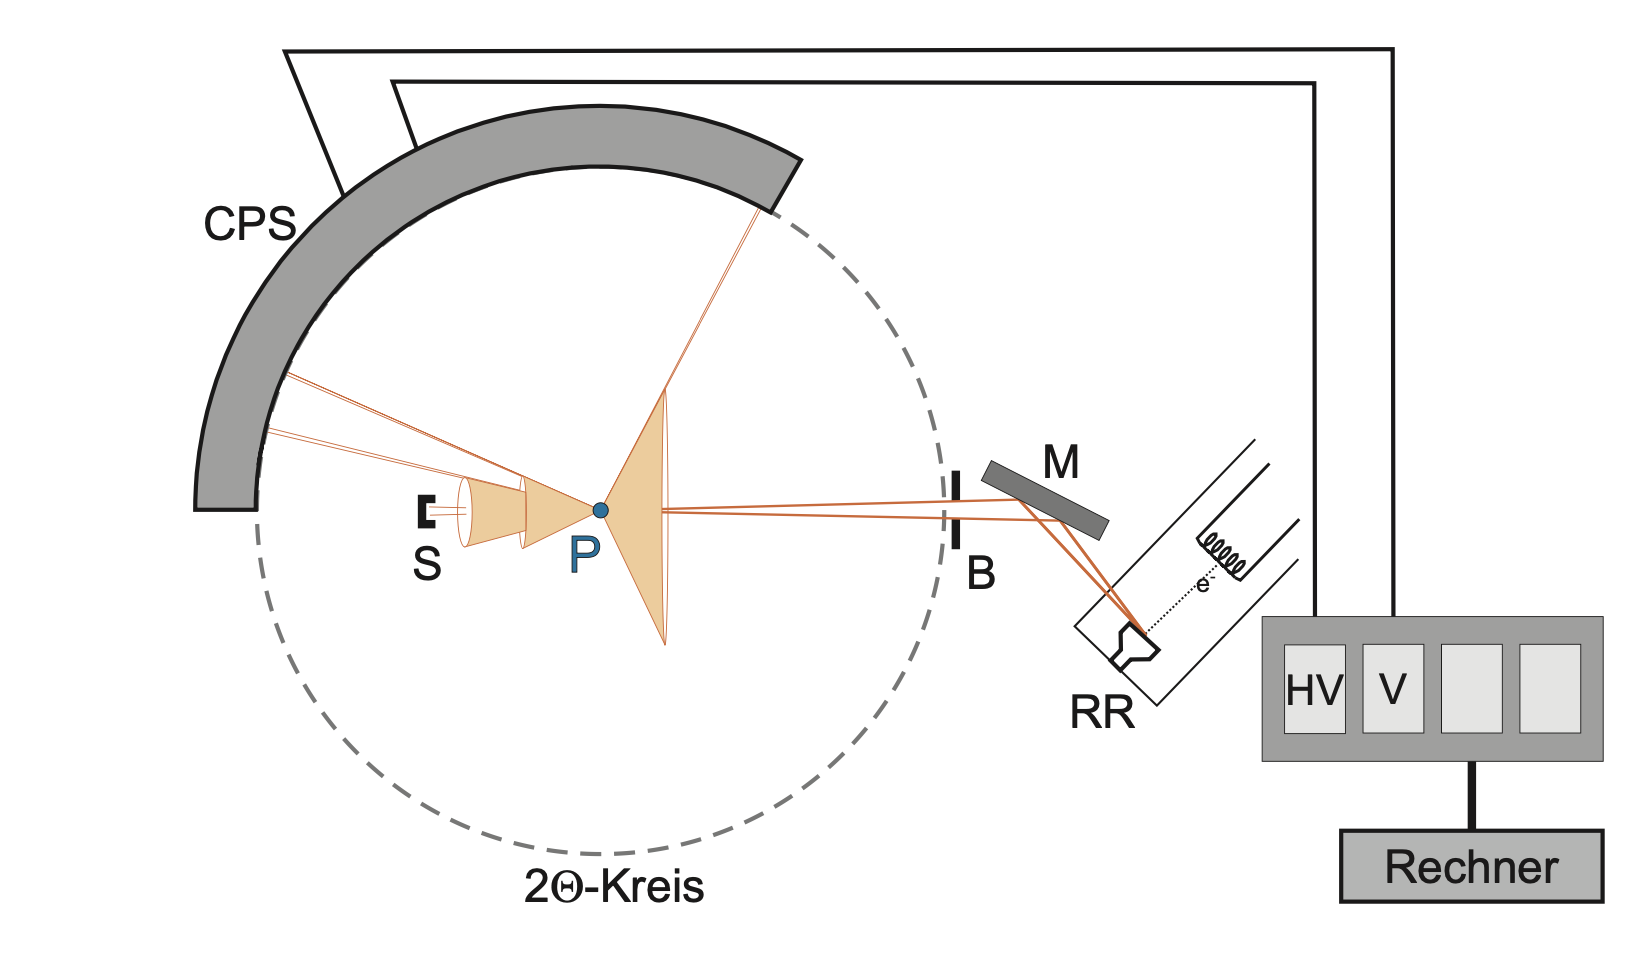
\includegraphics[width=0.73\textwidth]{Aufbau2.png}
    \caption{Skizze des Versuchsaufbaus zur Röntgenstrahlbeugung. Die Hauptbestandteile und deren 
    Funktionsweise sind im Haupttext beschrieben. Die Grafik wurde der Versuchsanleitung entnommen \cite{Anleitung}.}
    \label{fig:vers2}
\end{figure}\FloatBarrier

Die Röntgenstrahlung wird mithilfe einer Kupfer-Anode erzeugt. Für diesen Versuchsteil wird monochromatische Strahlung benötigt, die durch einen entlang der (111)-Ebene geschnitteten Germanium-Kristall erzeugt wird. Der Kristall dient also als Monochromator M. Die Röntgenstrahlung fällt auf die Pulverprobe, die sich in einer Kapillare P befindet. Die einzelnen Kristalle sind hierin regellos orientiert. Hinter der Probe befindet sich ein gekrümmter, ortsauflösender Detektor CPS, der die gebeugte Strahlung simultan in einem Winkelbereich von etwa $\SI{0}{\degree}$ bis $\SI{120}{\degree}$ misst. Zusätzlich befindet sich direkt hinter der Probe ein Primärstrahlfänger S, so dass wirklich nur gebeugte Strahlung den Detektor erreicht.\\
Zuerst muss die Probe präpariert werden. Dafür wird gewöhnliches Kochsalz für etwa 20 Minuten in einem Mörser zerkleinert und anschließend in eine Kapillare mit Durchmesser $d = \SI{1}{\milli\metre}$ gefüllt. Anschließend wird die Kapillare abgeschmolzen und in einem Messinghalter befestigt. Zum richtigen Zentrieren wird die Kapillare nun mit Hilfe von Rotationswiegen und Translationsschlitten unter dem Mikroskop so zentriert, dass sich die Kapillare bei späterer Drehung im Diffraktometer bei Drehung des Goniometerkopfes um die $\Omega$-Achse gleichzeitig um ihre eigene Achse dreht. Anschließend wird der Goniometerkopf auf der $\Omega$-Achse des Diffraktiometers montiert und der Motor angeschaltet. Die Röntgenröhre wird mit folgenden Werten betrieben:
\begin{equation}
    I = \SI[]{30}[]{\milli\ampere}, \qquad U = \SI[]{40}[]{\kilo\volt}
\end{equation}.\\
Das Diffraktogramm wird nun für eine knappe halbe Stunde gemessen. Längere Messzeiten würden nur eine geringe Verbesserung der Statistik bringen, da diese nur mit $\sqrt{N}$ eingeht. Deshalb kann bereits nach einer so kurzen Zeit das Messen aufgehört werden.\\
Bedient wird das Diffraktometer mit dem Computer und der Software GUF15. 